%% 
%% Official Elsevier elsarticle template integration.
%% Based on the local Elsevier Elsarticle Bundle in ../../elsarticle/.
%% Article content below \begin{document} is preserved from the source manuscript.
%%
\documentclass[preprint,12pt]{elsarticle}

%% Use the option review to obtain double line spacing
%% \documentclass[preprint,review,12pt]{elsarticle}

%% Use the options 1p,twocolumn; 3p; 3p,twocolumn; 5p; or 5p,twocolumn
%% for a journal layout:
%% \documentclass[final,1p,times]{elsarticle}
%% \documentclass[final,1p,times,twocolumn]{elsarticle}
%% \documentclass[final,3p,times]{elsarticle}
%% \documentclass[final,3p,times,twocolumn]{elsarticle}
%% \documentclass[final,5p,times]{elsarticle}
%% \documentclass[final,5p,times,twocolumn]{elsarticle}

%% The amssymb package provides various useful mathematical symbols
\usepackage{amssymb}
%% The amsmath package provides various useful equation environments.
\usepackage{amsmath}

%% Manuscript-specific packages required by existing tables, figures and links.
\usepackage{microtype}
\usepackage{ragged2e}
\usepackage{booktabs}
\usepackage{tabularx}
\usepackage{array}
\usepackage{xurl}
\usepackage[hypertexnames=false]{hyperref}
\pdfstringdefDisableCommands{%
  \def\corref#1{}%
  \def\cortext#1#2{}%
  \def\ead#1{}%
}
\usepackage{float}

\makeatletter
\setlength{\@fptop}{0pt}
\setlength{\@fpsep}{12pt}
\setlength{\@fpbot}{0pt plus 1fil}
\makeatother
\renewcommand{\topfraction}{0.95}
\renewcommand{\bottomfraction}{0.95}
\renewcommand{\textfraction}{0.06}
\renewcommand{\floatpagefraction}{0.80}
\setlength{\textfloatsep}{14pt plus 3pt minus 3pt}
\setlength{\floatsep}{12pt plus 3pt minus 3pt}
\setlength{\intextsep}{12pt plus 3pt minus 3pt}


\journal{Results in Engineering}

\begin{document}

\begin{frontmatter}

\title{Leakage-safe and calibration-aware model-threshold selection for multi-sensor robotic-arm anomaly diagnosis}

\author[aff1]{Haochen Li}
\author[aff1,aff2]{Junhao Wei}
\author[aff1]{Dexing Yao}
\author[aff1]{Yifu Zhao}
\author[aff1]{Yanxiao Li}
\author[aff1]{Zhaoyan Mai}
\author[aff1]{Jiamu Yu}
\author[aff1]{Baili Lu}
\author[aff3]{Sio-Kei Im}
\author[aff1]{Xu Yang}
\author[aff1]{Yapeng Wang\corref{cor1}}
\ead{yapengwang@mpu.edu.mo}
\cortext[cor1]{Corresponding author.}

\affiliation[aff1]{organization={Faculty of Applied Sciences, Macao Polytechnic University}, city={Macao}, postcode={999078}, country={China}}
\affiliation[aff2]{organization={Pazhou Lab (Huangpu)}, city={Guangzhou}, postcode={510555}, country={China}}
\affiliation[aff3]{organization={Macao Polytechnic University}, city={Macao}, postcode={999078}, country={China}}


\begin{abstract}
Multi-sensor robotic-arm anomaly diagnosis requires more than accurate fault classification: deployable monitoring also needs leakage-safe evaluation, validation-only threshold calibration and explicit false-alarm and missed-detection evidence. This paper evaluates a calibration-aware model-threshold selection framework under segment-, file- and run-level split protocols with train-only preprocessing and test-only final reporting. Across the evaluated strategy-validation scenarios, Fixed-\allowbreak LightGBM remained the strongest balanced default (macro-F1 0.785, PR-AUC 0.877, FAR 0.169, MDR 0.240), while objective-specific framework strategies exposed useful operating tradeoffs: Framework-\allowbreak Safety reduced MDR to 0.154 at FAR 0.322, and Framework-\allowbreak Low-\allowbreak False-\allowbreak Alarm reduced FAR to 0.087 at MDR 0.365; the balanced-utility difference over Fixed-\allowbreak LightGBM was not statistically significant. Label-budget analysis showed that normal-only and low-label calibration remain difficult, and robustness/domain-shift results indicate that the framework audits transfer risk rather than solving it. The contribution is an auditable engineering decision protocol for model-threshold selection. It links leakage-safe evaluation, validation-only calibration, FAR/MDR operating costs and prepared-input latency evidence without replacing strong fixed baselines.
\end{abstract}

\begin{keyword}
Robotic-arm anomaly diagnosis \sep model-threshold selection \sep leakage-safe evaluation \sep threshold calibration \sep false alarm rate \sep missed detection rate \sep deployment-oriented benchmarking
\end{keyword}

\end{frontmatter}


\section{Introduction}

Industrial robots and robotic arms are increasingly monitored through multiple sensor streams, including motion, current, vibration, torque and acoustic channels \cite{Chandola2009Survey,Pimentel2014NoveltyDetection,BlazquezGarcia2021TimeSeriesSurvey,Narayanan2018IndustrialArm}. These signals can expose collisions, abnormal loads, speed-related faults or early degradation, but anomaly diagnosis in this setting is an engineering operating decision rather than a static label-assignment problem. A false alarm can stop production, trigger unnecessary inspection or reduce operator trust. A missed detection can leave a safety or maintenance risk unresolved. A useful evaluation must therefore make false alarm rate (FAR), missed detection rate (MDR), threshold calibration and deployment latency visible alongside ranking metrics such as PR-AUC.

The credibility of such an evaluation depends on protocol design and reproducible implementation detail. Randomly splitting overlapping windows can leak near-duplicate temporal segments across training and test partitions. Tuning thresholds with test labels can also convert a benchmark into an optimistic operating-point search. These issues are particularly important for robotic-arm monitoring, where recordings are structured by runs, files, loads and target conditions, and where domain shift should be audited rather than treated as solved by a title-level claim. A deployment-facing benchmark should split by segment, file or run unit, fit normalization only on the training split and reserve test labels for final reporting rather than threshold selection.

A second limitation of ordinary benchmarks is that they typically ask which model has the highest average score. That question is necessary but insufficient for deployment. A safety-critical monitor, a production line with high nuisance-alarm cost, a low-label calibration setting and a prepared-input low-latency candidate-selection setting can require different model-threshold choices even when the same candidate models are available. The engineering question is therefore not only which model is strong, but which model-threshold pair should be selected under a stated operating cost and how much regret remains when that choice is evaluated on a held-out test set.

This study evaluates a leakage-safe and calibration-aware engineering framework for robotic-arm multi-sensor anomaly diagnosis. The framework compares fixed single-model strategies with validation-selected framework strategies using real benchmark outputs from IMAD-DS \cite{Augusti2024IMADDS}, RoAD as a secondary reference \cite{Gaiardelli2023RoAD} and related readiness datasets where appropriate. It treats model and threshold selection as an auditable decision layer around a candidate pool, not as a new detector. The study reports FAR, MDR, PR-AUC, regret, average rank, label-budget sensitivity, robustness and latency while preserving the strength of Fixed-\allowbreak LightGBM as an important empirical finding.

The study is organized around three research questions. \textbf{RQ1} asks how validation-only model-threshold selection compares with fixed model strategies in operating utility and regret, particularly relative to the strongest fixed baseline. \textbf{RQ2} asks under which operating objectives the framework improves over Fixed-\allowbreak LightGBM and where Fixed-\allowbreak LightGBM remains the better default. \textbf{RQ3} asks how deployment conclusions change with label budget, missing sensors, domain shift and latency constraints.

This paper makes three engineering contributions. First, it provides a leakage-safe and calibration-aware deployment protocol for robotic-arm anomaly diagnosis, combining segment/file/run-level splits, train-only preprocessing, validation-only thresholding, no test-set threshold tuning and no random overlapping-window split. Second, it evaluates a cost-aware model-threshold selection framework for deployment-oriented anomaly diagnosis, comparing fixed model strategies with validation-selected framework strategies across balanced, safety, low-false-alarm, robust, deployment and label-budget utilities, with FAR/MDR, regret and latency evidence. Third, it provides a reproducible engineering evaluation across label budget, robustness, domain shift and deployment constraints, including main benchmark results, FAR/MDR tradeoffs, label-budget sensitivity, robustness/domain-shift stress, latency analysis, scenario-specific guidance and honest negative findings. The boundary is deliberately explicit: the framework is a validation-calibrated decision protocol over existing detectors and does not claim a new anomaly detection algorithm or universal model dominance.

\begin{table}[!htbp]
\centering
\footnotesize
\setlength{\tabcolsep}{4pt}
\renewcommand{\arraystretch}{1.12}
\caption{Contribution-to-evidence mapping. The table summarizes how each engineering contribution is supported by the protocol design, results and discussion.}
\label{tab:contribution-evidence}
\begin{tabularx}{\linewidth}{@{}>{\RaggedRight\arraybackslash}p{0.24\linewidth}>{\RaggedRight\arraybackslash}p{0.32\linewidth}>{\RaggedRight\arraybackslash}p{0.20\linewidth}>{\RaggedRight\arraybackslash}X@{}}
\toprule
Contribution & Evidence in manuscript & Main support & Evidence scope \\
\midrule
Leakage-safe and calibration-aware deployment protocol & Segment/file/run-level split, train-only preprocessing, validation-only thresholding, no random overlapping-window split and no test-set threshold tuning & Data and Protocols; Table~\ref{tab:dataset-inclusion}; protocol risk section; Fig.~\ref{fig:framework-workflow} & Evaluated under the reported split/protocol design and dataset roles \\
Cost-aware model-threshold selection for deployment-oriented anomaly diagnosis & Fixed model strategies compared with validation-selected framework strategies under balanced, safety, low-false-alarm, robust, deployment and label-budget utilities & Strategy utility definitions; Procedure~1; Table~\ref{tab:statistical-evidence}; FAR/MDR and latency results & Applies to the candidate model pool and validation/calibration quality used in this study \\
Reproducible engineering evaluation across deployment constraints & Main benchmark, FAR/MDR tradeoff, label-budget, robustness/domain-shift, latency and scenario guidance with negative findings retained & Results; application scenario mapping; limitations & Supports deployment-oriented evidence synthesis across the evaluated datasets and constraints \\
\bottomrule
\end{tabularx}
\end{table}


\section{Related Work}



\subsection{Robotic and industrial anomaly diagnosis}



Robotic and industrial anomaly diagnosis has been studied for collaborative robot monitoring, industrial arm applications and production-line anomalies \cite{Narayanan2018IndustrialArm,Gaiardelli2023RoAD}. These applications share a deployment constraint: an alarm is not merely a label prediction but an operational decision. Existing datasets such as IMAD-DS and RoAD provide useful real-world contexts, but they also require careful protocol design because operating conditions, domain shifts and artifacts can shape the apparent difficulty of the task \cite{Augusti2024IMADDS,Gaiardelli2023RoAD}. Existing work often emphasizes detection performance, while fewer studies enforce leakage-safe split units and validation-only threshold selection for deployment decisions.



\subsection{Multi-sensor time-series anomaly detection}



Multi-sensor time-series anomaly detection often uses temporal reconstruction, sequence prediction, graph structure or density-based scoring \cite{BlazquezGarcia2021TimeSeriesSurvey,Malhotra2016LSTMEncDec,Audibert2020USAD}. LSTM encoder-decoder models and USAD-style autoencoder methods are representative reconstruction-based baselines for multivariate time series \cite{Malhotra2016LSTMEncDec,Audibert2020USAD}. These methods can be attractive when anomaly labels are limited, but their operating behavior still depends on score calibration and threshold selection. They provide anomaly scores, but deployable operating points still depend on calibration and threshold selection.



\subsection{Tree-based and statistical baselines}



Tree-based models remain strong engineering baselines for window-level statistical features. LightGBM implements efficient gradient boosting decision trees \cite{Ke2017LightGBM}, XGBoost provides scalable tree boosting \cite{Chen2016XGBoost}, and RandomForest is a classic ensemble of randomized decision trees \cite{Breiman2001RandomForests}. IsolationForest is a commonly used unsupervised anomaly detector based on isolation rather than density estimation \cite{Liu2008IsolationForest,Liu2012IsolationBased}. In the present results, Fixed-\allowbreak LightGBM remains a particularly strong default, and this strength is retained as a central finding. Strong tree baselines motivate an audit framework that validates and calibrates them rather than replacing them.



\subsection{Threshold calibration and leakage-safe evaluation}



Threshold calibration is central to deployable anomaly detection and is closely related to broader calibration and benchmark-reliability concerns in machine learning and time-series anomaly detection \cite{Guo2017Calibration,Wu2021TSADBenchmarksFlawed,Tatbul2018PrecisionRecallTS}. A model with good ranking metrics can still be unsuitable if its operating threshold produces excessive false alarms or missed detections. Conformal prediction and distribution-free calibration provide one family of calibration ideas \cite{Vovk2005Conformal,Lei2018Conformal}, while practical validation-only threshold selection is a simpler engineering route when labeled validation data are available. This paper uses validation-only thresholds and reports FAR/MDR operating behavior rather than optimizing thresholds on test labels. The present study combines leakage-safe split, train-only normalization and validation-only thresholding in one engineering protocol.



\subsection{Deployment-aware engineering evaluation}



Deployment-aware evaluation should consider label budgets, missing sensors, domain shift, latency, model size and the cost of false alarms or missed detections \cite{Sokolova2009PerformanceMeasures,Elkan2001CostSensitive,Drummond2006CostCurves,Sculley2015TechnicalDebt,Breck2017MLTestScore,Amershi2019SE4ML}. These considerations connect anomaly detection to model selection under constraints: the deployable choice is the model-threshold pair that satisfies a stated operating preference, not necessarily the model with the highest average score. This view is also aligned with engineering decision support, where the justification for a deployed system depends on traceable evidence, calibration data and operational constraints. The present framework formalizes these constraints as strategy-level utility functions and uses them to separate benchmark comparison from pre-deployment decision making. It combines FAR/MDR, regret, latency, label budget and robustness as model-threshold selection evidence.



\section{Data and Leakage-Safe Protocols}



The primary dataset is IMAD-DS RoboticArm in raw-window form. IMAD-DS contains robotic-arm and brushless-motor data under operational and environmental domain shifts, with microphone, accelerometer and gyroscope channels recorded under controlled industrial conditions \cite{Augusti2024IMADDS}. The raw-window RoboticArm adapter provides the main evidence because it preserves temporal multi-sensor structure while still supporting leakage-safe segment-level split rules. In the current processed benchmark, this view contains 4364 windows and seven raw sensor channels across 25 recorded conditions. It is therefore the main source for binary detection, source-to-target transfer, leave-target-weight35-out stress, missing-sensor robustness, noise stress, label-budget and latency analyses.

IMAD-DS RoboticArm segment-level features are used as a granularity comparison. This view contains compact statistical summaries rather than raw windows, and it tests whether engineering conclusions are stable when the same underlying robotic-arm data are represented at a segment-feature level. IMAD-DS BrushlessMotor is treated as secondary industrial validation when the adapter and labels support the corresponding protocol. It is useful for checking whether the framework carries beyond the robotic-arm subset, but it is not used to replace the main robotic-arm evidence. RoAD is retained only as a secondary sanity or stress reference because earlier audits identified confounding and artifact risks \cite{Gaiardelli2023RoAD}. NIST UR and KUKA are not used as primary binary anomaly evidence in the main analysis when labels, access or data structure do not support the same binary protocols. This conservative role assignment keeps readiness datasets separate from the main robotic-arm binary evidence when their labels or protocol structure are not fully aligned with the primary diagnostic task.

\begin{table}[!htbp]
\centering
\scriptsize
\setlength{\tabcolsep}{3pt}
\renewcommand{\arraystretch}{1.08}
\caption{Dataset inclusion and exclusion rationale. The table separates primary evidence from secondary checks and readiness-only datasets.}
\label{tab:dataset-rationale}
\label{tab:dataset-inclusion}
\begin{tabularx}{\linewidth}{@{}>{\RaggedRight\arraybackslash}p{0.17\linewidth}>{\RaggedRight\arraybackslash}p{0.28\linewidth}>{\RaggedRight\arraybackslash}p{0.22\linewidth}>{\RaggedRight\arraybackslash}X@{}}
\toprule
Dataset & Used for & Not used for & Rationale \\
\midrule
IMAD-DS RoboticArm & Primary binary detection; source-to-target; leave-target-weight35-out; missing sensor/noise; label budget; latency. & Not applicable. & Labels and split units support the main robotic-arm task; multi-sensor robotic-arm data. \\
IMAD-DS BrushlessMotor & Secondary industrial validation where adapter and labels support protocol. & Primary robotic-arm claim. & Different asset type; useful as secondary industrial check. \\
RoAD & Secondary sanity/stress reference. & Main binary claim. & Confounding/artifact risk. \\
NIST UR & Readiness/exclusion note only, if applicable. & Primary binary anomaly evidence. & Label/access/protocol mismatch. \\
KUKA & Readiness/exclusion note only, if applicable. & Primary binary anomaly evidence. & Label/access/protocol mismatch. \\
\bottomrule
\end{tabularx}
\end{table}




All protocols are designed to reduce leakage. The split unit is segment, file or run identifier wherever available. Window-level random splitting is not used. Normalization is fit on training data only. Model thresholds and framework strategy choices are selected using validation or calibration data only. Test labels are used only for final evaluation. The raw-window protocols retain temporal structure for time-series baselines, while segment-level protocols provide a separate statistical-feature granularity check. This separation is important because strong tree models can perform well on compact statistical summaries, whereas raw-window models expose different latency and calibration behavior.



The protocol set includes main binary classification, source-to-target domain shift, leave-target-weight35-out stress testing, missing-sensor settings, noise stress, label-budget settings and latency benchmarking. Table~\ref{tab:experiment-design} summarizes how these blocks are mapped to datasets, candidate strategies and engineering purposes. Each result row carries provenance fields including dataset, protocol, seed, method, train/validation/test counts, test normal/anomaly counts, provenance timestamp and result artifact identifier. No synthetic result is used.

\begin{table}[!htbp]
\centering
\footnotesize
\setlength{\tabcolsep}{4pt}
\renewcommand{\arraystretch}{1.12}
\caption{Experiment design matrix. The table summarizes the main protocol blocks; all blocks use leakage-safe split units and validation-only calibration.}
\label{tab:experiment-design}
\begin{tabularx}{\linewidth}{@{}>{\RaggedRight\arraybackslash}p{0.15\linewidth}>{\RaggedRight\arraybackslash}p{0.25\linewidth}>{\RaggedRight\arraybackslash}p{0.18\linewidth}>{\RaggedRight\arraybackslash}p{0.16\linewidth}>{\RaggedRight\arraybackslash}X@{}}
\toprule
Block & Data and protocols & Model pool & Main metrics & Purpose \\
\midrule
Main benchmark & IMAD-DS RoboticArm raw-window and segment-level; BrushlessMotor if valid & Fixed baselines and framework strategies & macro-F1, PR-AUC, FAR, MDR & Primary diagnosis and granularity comparison \\
Operating constraints & Safety and low-false-alarm thresholds across IMAD-DS protocols & Framework-Safety, Framework-Low-False-Alarm, strong fixed baselines & FAR/MDR violations & Operating-point tradeoff analysis \\
Label budget & Normal-only, 5\%, 20\% and full validation budgets & Fixed and framework strategies & macro-F1, PR-AUC, FAR, MDR & Label-scarcity diagnosis \\
Robustness and shift & Missing sensors, noise, source-to-target and holdout settings & Fixed baselines, Framework-Robust and Framework-Balanced & degradation and utility & Stress and deployment reliability \\
Deployment & Per-window latency and model-size measurements & Tree, statistical and deep baselines; Framework-Deployment & latency and prepared-input deployment-screening utility & prepared-input screening feasibility \\
Guidance & Valid strategy-validation scenarios & Validation-selected strategies and fixed defaults & rank, regret and utility & Scenario-specific decision support \\
\bottomrule
\end{tabularx}
\end{table}


\subsection{Protocol risk and leakage control}

The protocol design is motivated by two common failure modes in time-series anomaly evaluation. The first is random overlapping-window splitting. When neighboring windows share most of their samples, a random split can place near-duplicates in both training and test partitions. The resulting test performance can reflect temporal memorization rather than generalization to unseen runs or operating conditions. The second is test-set threshold tuning. Because anomaly detectors often produce continuous scores, selecting a threshold using test labels directly optimizes the reported operating point and is not deployable in a new plant or robot cell.

The present benchmark controls these risks by separating the roles of training, validation and test data. Normalization statistics are fit on the training split only. Thresholds, operating points and framework strategy choices are selected only on validation or calibration data. Test labels are used only once, for final reporting. This design does not remove all dataset bias, but it makes the remaining assumptions visible: if a model performs well, it has done so under a split and calibration rule that could be reproduced before deployment.




\subsection{Implementation details and reproducibility}

The benchmark implementation separates raw-window and tabular segment protocols. For raw-window IMAD-DS RoboticArm experiments, tree models use statistical features extracted from train-only-normalized multivariate windows. The available raw-window feature extractor reports channel-wise mean, standard deviation, minimum, maximum and endpoint difference between the last and first sample in the window. No RMS, skewness, kurtosis or FFT/band-energy feature names are inferred here because they are not explicitly present in the available raw-window extractor artifact. AutoEncoder, LSTM-\allowbreak AE and USAD consume normalized multivariate windows directly rather than the tree-feature table. Segment-level and secondary tabular datasets use numeric columns from the unified CSV adapters after excluding metadata and label fields. Tabular scaling uses a \texttt{StandardScaler} fit on the training split only; raw-window normalization uses train-only channel statistics before validation and test transformations.

The processed IMAD-DS RoboticArm raw-window artifact contains 4364 windows and seven sensor channels. The main benchmark protocol reports 2508 training windows, 608 validation windows and 624 test windows, with 312 normal and 312 anomaly windows in the test split. The representative main binary split uses 3740 windows; the remaining 624 windows are not discarded, but are excluded from this split-level summary and retained in the processed artifact for protocol-specific analyses documented in the provenance files. Table~\ref{tab:split-accounting} summarizes this accounting distinction.

\input{tables/table_split_accounting_v19.tex}

The processed manuscript-level artifacts do not preserve sampling-rate, stride and overlap metadata. The results are therefore interpreted at the processed-window level rather than raw time resolution, and no unsupported raw-time sampling claims are made. Split units are segment, file or run identifiers wherever available.

The available configuration fixes five random seeds (7, 13, 23, 31 and 42), validation-only thresholding, train-only normalization and segment/file/run-level split units. Missing-sensor stress randomly drops channels and sets the selected channels to zero in validation/test stress protocols, with 10\% and 20\% channel-drop settings in the benchmark runner. Noise stress adds Gaussian noise scaled by channel standard deviation, with 0.02 and 0.05 scale settings in the available implementation. Label-budget settings include normal-only, 5\%, 20\% and full validation-label budgets. The anomaly/fault class is treated as the positive class for PR-AUC, FAR, MDR and threshold calibration.

The candidate model settings are summarized in Table~\ref{tab:model-parameters}. These settings are reported as reproducible baseline configurations for model-threshold evaluation, not as optimized architecture claims.

\input{tables/table_model_parameters_v19.tex}

Candidate thresholds are generated on validation or calibration scores using predeclared threshold strategies: best-F1, Youden's index, target FAR of 0.05, 0.10 and 0.15, target recall of 0.80, 0.90 and 0.95, and missed-detection/false-alarm cost ratios of 2:1, 5:1 and 10:1. Test labels are never used for threshold selection. In the normal-only label-budget condition, anomaly validation labels are unavailable; thresholds are therefore based on normal-score quantiles or unsupervised calibration rules, and supervised tree models that require anomaly labels for training are skipped rather than tuned with macro-F1. The 5\%, 20\% and full label-budget settings can use labeled validation subsets for utility-based threshold selection.

Latency values are measured as model prediction latency on prepared features or prepared windows and are reported per window. They are not end-to-end robot-cell latency and do not include sensor I/O, robot middleware, alarm handling or operator response. For tree and statistical models, feature extraction and train-only normalization are upstream of the timed prediction path in the available artifacts. Deep reconstruction scores are computed on prepared normalized windows. The exact processor/GPU model, warm-up count and number of repetitions are not preserved in the available latency artifacts. Table~\ref{tab:repro-config} summarizes the reported configuration and interpretation limits.

\begin{table}[!htbp]
\centering
\scriptsize
\setlength{\tabcolsep}{3pt}
\renewcommand{\arraystretch}{1.12}
\caption{Reproducibility configuration and interpretation limits from available artifacts.}
\label{tab:repro-config}
\begin{tabularx}{\linewidth}{@{}>{\RaggedRight\arraybackslash}p{0.15\linewidth}>{\RaggedRight\arraybackslash}p{0.33\linewidth}>{\RaggedRight\arraybackslash}p{0.21\linewidth}>{\RaggedRight\arraybackslash}X@{}}
\toprule
Component & Reported setting & Evidence/source & Interpretation or limitation \\
\midrule
Input features & Tree models use channel-wise mean, standard deviation, minimum, maximum and endpoint difference; deep baselines use normalized multivariate windows. & raw-window adapter; benchmark runner & No additional RMS, skewness, kurtosis or FFT/band-energy features are inferred from unavailable artifacts. \\
Processed windows & IMAD-DS RoboticArm raw-window artifact contains 4364 windows and seven channels; main split reports 2508 train, 608 validation and 624 test windows with 312 normal and 312 anomaly test windows. & strategy selection log; manuscript result artifacts & Sampling-rate, stride and overlap metadata are not preserved in manuscript-level outputs; results are interpreted at processed-window level. \\
Split and preprocessing & Segment/file/run-level splitting with train-only normalization and validation-only threshold selection. & benchmark runner; strategy validation script & Test labels are used only for final reporting. \\
Stress protocols & Missing-sensor stress uses 10\textbackslash{}\% and 20\textbackslash{}\% channel-drop settings; noise stress uses Gaussian scale 0.02 and 0.05. & benchmark runner & Stress results are benchmark robustness evidence, not online fault-injection trials. \\
Model settings & LightGBM 70 estimators/lr 0.06/31 leaves; XGBoost 60 estimators/depth 4/lr 0.06; RandomForest 80 trees/depth 10; compact AE/LSTM-AE/USAD baselines trained for three epochs with AdamW lr $10^{-3}$ and batch size 128. & benchmark runner & Settings define reproducible baselines rather than optimized architecture claims. \\
Threshold grid & Validation-only best-F1, Youden, target FAR 0.05/0.10/0.15, target recall 0.80/0.90/0.95 and cost ratios 2:1, 5:1 and 10:1. & threshold sensitivity files; strategy validation script & Normal-only label-budget calibration uses normal-score rules rather than anomaly-label macro-F1 tuning. \\
Latency & Prepared-input prediction latency is reported per window; tree feature extraction, sensor I/O, robot middleware, alarm handling and operator response are excluded. & latency/deployment result table; benchmark runner & Hardware, warm-up and repetition metadata are not preserved; latency is descriptive prepared-input timing only. \\
\bottomrule
\end{tabularx}
\end{table}


\section{Benchmark Models and Framework Strategies}



The fixed model strategies use one model family across all evaluated scenarios. They include Fixed-\allowbreak LightGBM, Fixed-\allowbreak XGBoost, Fixed-\allowbreak RandomForest, Fixed-\allowbreak IsolationForest, Fixed-\allowbreak AutoEncoder, Fixed-\allowbreak LSTM-\allowbreak AE and Fixed-\allowbreak USAD. These are benchmark strategies, not components of a proposed method.



The framework strategies are not new predictive models. They select a candidate model and threshold using validation or calibration data. Framework-\allowbreak Best-\allowbreak F1 selects the validation macro-F1 optimum. Framework-\allowbreak Balanced maximizes macro-F1 minus FAR and MDR. Framework-\allowbreak Safety increases the penalty on missed detections. Framework-\allowbreak Low-\allowbreak False-\allowbreak Alarm increases the penalty on false alarms. Framework-\allowbreak Robust considers robustness degradation where validation robustness metrics are available. Framework-\allowbreak Deployment includes latency and model-size penalties. Framework-\allowbreak Label-\allowbreak Budget evaluates normal-only, 5\%, 20\% and full validation-label budgets.

Operationally, the framework input is a pool of already implemented candidate models, their validation scores, calibrated thresholds, latency and model-size estimates, and protocol metadata. The output is not a new score function. It is a selected model, selected threshold strategy and deployment recommendation for the specified engineering objective. This distinction is central to the claim. A deployment team may select the same LightGBM model in many settings, but the framework records why it was selected, which threshold was used, which validation utility justified the decision and how much regret remained relative to the non-deployable oracle.

\begin{figure}[!htbp]
\centering
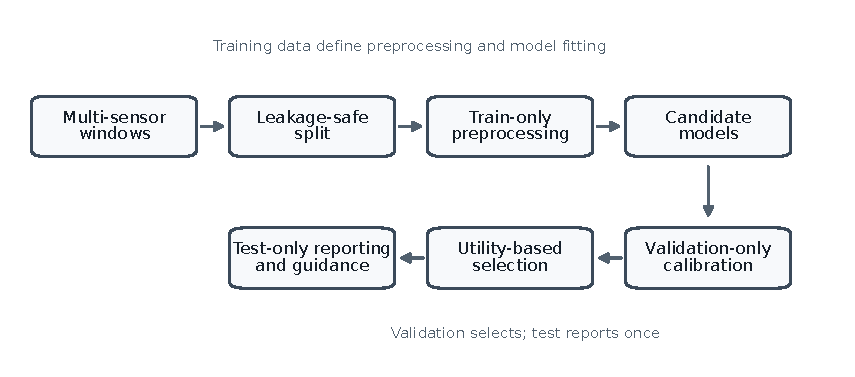
\includegraphics[width=0.95\linewidth]{figures/fig1_workflow_v19.pdf}
\caption{Leakage-safe and calibration-aware model-threshold selection workflow. Data are split by segment, file or run unit. Preprocessing is fit on the training split only, model-threshold selection is performed using validation/calibration data only, and held-out test labels are used once for final reporting. The workflow is a decision layer around existing detectors, not a new anomaly score.}
\label{fig:framework-workflow}
\end{figure}




Oracle-\allowbreak Best-\allowbreak Test-\allowbreak Utility is included only as a retrospective theoretical upper-bound reference. It is selected by scenario-level utility rather than by independently maximizing each reported metric, which is why it should not be interpreted as a metric-wise oracle. It is non-deployable because it uses test-set outcomes for retrospective upper-bound analysis and must not be used for model or threshold selection.


\subsection{Strategy utilities and validation-only selection}

Let the candidate model pool be
\begin{equation}
\begin{aligned}
\mathcal{M}=\{&\mathrm{LightGBM},\ \mathrm{XGBoost},\ \mathrm{RandomForest},\ \mathrm{IsolationForest},\\
&\mathrm{AutoEncoder},\ \mathrm{LSTM\mbox{-}AE},\ \mathrm{USAD}\}.
\end{aligned}
\end{equation}
For a model $m\in\mathcal{M}$, let $\mathcal{T}_{m}$ denote the set of candidate thresholds available after validation or calibration. The validation split $D_{\mathrm{val}}$ is used for model-threshold selection, while the held-out test split $D_{\mathrm{test}}$ is reserved for final reporting. For an engineering objective $k$, the selected model-threshold pair is
\begin{equation}
(m^{*}_{k},\tau^{*}_{k})=\arg\max_{m\in\mathcal{M},\tau\in\mathcal{T}_{m}} U_{k}(m,\tau;D_{\mathrm{val}}),
\label{eq:validation-selection}
\end{equation}
where $U_k$ is the predeclared utility for objective $k$. Equation~\ref{eq:validation-selection} defines a decision rule over existing detectors and thresholds; it does not define a new anomaly score. Once $(m^{*}_{k},\tau^{*}_{k})$ has been selected, all reported test metrics are computed once on $D_{\mathrm{test}}$.

The utilities encode operating preferences rather than test-set-tuned weights:
\begin{align}
U_{\mathrm{balanced}} &= \mathrm{macroF1}-\mathrm{FAR}-\mathrm{MDR},\label{eq:ubalanced}\\
U_{\mathrm{safety}} &= \mathrm{macroF1}-2\,\mathrm{MDR}-0.5\,\mathrm{FAR},\label{eq:usafety}\\
U_{\mathrm{lowFA}} &= \mathrm{macroF1}-2\,\mathrm{FAR}-0.5\,\mathrm{MDR},\label{eq:ulowfa}\\
U_{\mathrm{deploy}} &= \mathrm{macroF1}-\mathrm{FAR}-\mathrm{MDR}-P_{\mathrm{latency}}-P_{\mathrm{size}},\label{eq:udeploy}\\
U_{\mathrm{robust}} &= U_{\mathrm{detection}}-\Delta_{\mathrm{robust}},\label{eq:urobust}\\
U_{\mathrm{label}}(b) &= \mathrm{macroF1}-\mathrm{FAR}-\mathrm{MDR}\quad\text{under label budget }b.\label{eq:ulabel}
\end{align}
The deployment penalties are implementation-defined but explicit: $P_{\mathrm{latency}}=0.05\log(1+\ell_m)/\log(1+\ell_{\max})$, where $\ell_m$ is the prepared-input prediction latency for model $m$, and $P_{\mathrm{size}}=0.05\log(1+s_m)/\log(1+s_{\max})$, where $s_m$ is the model-size estimate. The maxima $\ell_{\max}$ and $s_{\max}$ are computed over the benchmark candidate rows before final reporting. Prepared-input deployment-screening utility is therefore a descriptive operating score over prepared-input prediction cost, not an end-to-end robot-cell timing guarantee. The robust selection utility uses $\Delta_{\mathrm{robust}}=\max(0,\mathrm{macroF1}_{\mathrm{clean,val}}-\mathrm{macroF1}_{\mathrm{stress,val}})$ when a clean validation counterpart is available; selected test summaries report robustness evidence through the corresponding stressed-scenario metrics. The label-budget variable $b$ denotes the available validation-label setting, such as normal-only, 5\%, 20\% or full validation. These utilities are deliberately simple so that the operating preference is inspectable before test evaluation. The label-budget utility is an evaluation condition, not evidence that label-budget superiority has been achieved.

\begin{center}
\setlength{\fboxsep}{7pt}
\fbox{%
\begin{minipage}{0.94\linewidth}
\small
\textbf{Procedure 1. Leakage-safe calibration-aware model and threshold selection}\par
\vspace{2pt}
\textbf{Input:} multi-sensor robotic-arm data; split units; candidate model pool $\mathcal{M}$; engineering objective $k$; train, validation/calibration and test splits.\par
\textbf{Output:} selected model $m^{*}_{k}$; selected threshold $\tau^{*}_{k}$; operating strategy; final test metrics; deployment caution.\par
\vspace{2pt}
\begin{enumerate}
\setlength{\itemsep}{1pt}
\setlength{\parskip}{0pt}
\item Split data by segment, file or run unit.
\item Fit normalization on training data only.
\item Train each candidate model on the training data.
\item Generate validation scores for each candidate model.
\item Calibrate candidate thresholds on validation/calibration data.
\item Compute $U_k(m,\tau;D_{\mathrm{val}})$ for each model-threshold pair.
\item Select $(m^{*}_{k},\tau^{*}_{k})$ using validation utility only.
\item Evaluate the selected pair once on held-out $D_{\mathrm{test}}$.
\item Report FAR, MDR, PR-AUC, regret, latency and deployment guidance.
\end{enumerate}
\textit{This procedure is an evaluation and decision workflow, not a new detector.}
\end{minipage}}
\end{center}

\section{Evaluation Metrics and Statistical Analysis}



The evaluation reports macro-F1, weighted-F1, AUROC, PR-AUC, FAR, MDR and FAR@95\%Recall. Macro-F1 and PR-AUC summarize detection quality, while FAR and MDR express operational costs. FAR@95\%Recall indicates the false-alarm burden required to reach a high-recall operating point; the core summary is reported in Table~\ref{tab:far95-core}.



Strategy-level performance is summarized by average rank, win count, top-2 count and regret relative to Oracle-\allowbreak Best-\allowbreak Test-\allowbreak Utility. For metrics where larger values are better, regret is the gap between the oracle metric and the selected strategy. For metrics where smaller values are better, regret is the selected strategy value minus the oracle value. Engineering utilities are reported for balanced, safety, low-false-alarm, robust, deployment and label-budget settings.



Statistical comparisons use paired tests where matched scenario-level results are available. Each paired sample corresponds to one unique dataset--protocol--seed--scenario comparison when the same evaluation unit is available for both strategies. A scenario-level result is defined by the dataset, protocol family, seed, strategy pair, utility objective and metric aggregation unit. Individual windows are not treated as independent statistical samples.

The paired tests should be read as benchmark evidence summaries rather than proof of independent field trials. Multiple scenario-level samples can share the same dataset, protocol family and held-out split structure, and results that share the same underlying test split but differ in threshold or strategy remain statistically dependent. The Wilcoxon signed-rank test is emphasized because scenario-level utility differences need not be normally distributed. Unadjusted Wilcoxon p-values, effect sizes, wins/losses, sign tests and cluster-bootstrap details are provided in the Supplementary Material and the public reproducibility repository. Holm correction is applied to the prespecified Wilcoxon comparisons from the framework validation gate. The cluster bootstrap resamples 19 dataset--protocol groups with replacement, uses B=5000 replicates and reports percentile 95\% intervals. Because clusters share dataset--protocol families, these intervals are interpreted as benchmark evidence rather than independent field-trial uncertainty. Table~\ref{tab:statistical-evidence} therefore reports only the key columns needed for the main manuscript.

\begin{table}[!htbp]
\centering
\scriptsize
\setlength{\tabcolsep}{4.5pt}
\renewcommand{\arraystretch}{1.08}
\caption{Compressed statistical evidence for prespecified framework-versus-fixed comparisons. Each comparison uses $n=95$ paired scenario-level samples. Unadjusted Wilcoxon $p$-values, effect sizes and wins/losses are retained in the supplementary analysis files generated with this manuscript. Cluster intervals use dataset--protocol group resampling with replacement.}
\label{tab:statistical-evidence}
\begin{tabularx}{\linewidth}{@{}>{\RaggedRight\arraybackslash}p{0.27\linewidth}>{\RaggedRight\arraybackslash}p{0.14\linewidth}r r r >{\RaggedRight\arraybackslash}X@{}}
\toprule
Comparison & Objective & Mean diff. & Holm $p$ & Cluster 95\% CI & Result \\
\midrule
Balanced vs Fixed-LightGBM & balanced & 0.0020 & 0.1371 & [-0.016, 0.018] & small, not significant \\
Balanced vs Fixed-XGBoost & balanced & 0.0686 & 9.98e-10 & [0.037, 0.096] & framework advantage \\
Balanced vs Fixed-RandomForest & balanced & 0.1142 & 5.62e-10 & [0.071, 0.155] & framework advantage \\
Safety vs Fixed-LightGBM & safety & 0.0706 & 9.10e-08 & [0.013, 0.127] & framework advantage \\
Low-FA vs Fixed-LightGBM & low false alarm & 0.0946 & 2.10e-09 & [0.066, 0.125] & framework advantage \\
Deployment vs Fixed-XGBoost & deployment & 0.0603 & 9.98e-10 & [0.027, 0.087] & framework advantage \\
Deployment vs Fixed-RandomForest & deployment & 0.1175 & 4.11e-10 & [0.071, 0.163] & framework advantage \\
\bottomrule
\end{tabularx}
\end{table}


\begin{table}[!htbp]
\centering
\scriptsize
\setlength{\tabcolsep}{2.8pt}
\renewcommand{\arraystretch}{1.05}
\caption{Core FAR@95\%Recall summary. The metric reports the false-alarm burden needed to reach a high-recall operating point and is reported from existing strategy summaries rather than used for test-set threshold selection.}
\label{tab:far95-core}
\begin{tabularx}{\linewidth}{@{}>{\RaggedRight\arraybackslash}X*{4}{>{\centering\arraybackslash}p{0.105\linewidth}}@{}}
\toprule
Strategy & \shortstack{FAR@95\%\\Recall} & Std. & Macro-F1 & PR-AUC \\
\midrule
Framework-Balanced & 0.480 & 0.346 & 0.773 & 0.861 \\
Framework-Safety & 0.479 & 0.348 & 0.738 & 0.858 \\
Framework-Low-False-Alarm & 0.488 & 0.342 & 0.750 & 0.859 \\
Framework-Deployment & 0.485 & 0.345 & 0.770 & 0.859 \\
Fixed-LightGBM & 0.482 & 0.325 & 0.785 & 0.877 \\
Fixed-XGBoost & 0.515 & 0.309 & 0.761 & 0.861 \\
Fixed-RandomForest & 0.517 & 0.340 & 0.744 & 0.835 \\
\bottomrule
\end{tabularx}
\end{table}


The FAR@95\%Recall summaries are intentionally interpreted as operating-point stress evidence rather than as a primary ranking metric. FAR@95\%Recall remains high for all displayed strategies (0.480--0.517), indicating that high-recall operation would impose a substantial false-alarm burden. This reinforces the need for explicit operating-point selection rather than relying only on ranking metrics.





\section{Results}

The Results section answers the three research questions using the existing benchmark artifacts. RQ1 is addressed by the overall utility, regret and statistical summaries. RQ2 is addressed by FAR/MDR operating constraints and the comparison with Fixed-\allowbreak LightGBM. RQ3 is addressed through label-budget, robustness/domain-shift and latency/prepared-input screening analyses. The public repository supports reproduction of aggregate tables, statistical comparisons and figures from released result summaries, configuration files and command manifests. For third-party datasets whose redistribution is restricted or not verified, the repository provides official access instructions and reconstruction scripts rather than redistributing restricted dataset copies.



\subsection{Overall framework strategy comparison}



The fixed-model baseline comparison includes LightGBM, XGBoost, RandomForest, IsolationForest, AutoEncoder, LSTM-AE and USAD. The results retain these models as engineering baselines rather than treating any of them as a proposed method. In aggregate, the tree-based baselines, especially Fixed-\allowbreak LightGBM, provide the strongest default behavior, while deep reconstruction baselines remain useful comparison points but do not dominate FAR/MDR-constrained operation.

\begin{table}[!htbp]
\centering
\scriptsize
\setlength{\tabcolsep}{2pt}
\renewcommand{\arraystretch}{1.05}
\caption{Summary of fixed-model and framework strategies. Oracle-Best-Test-Utility is a theoretical upper bound and is not deployable.}
\label{tab:main-framework-strategy}
\begin{tabularx}{\linewidth}{@{}>{\RaggedRight\arraybackslash}X*{6}{>{\centering\arraybackslash}p{0.082\linewidth}}@{}}
\toprule
Strategy & Macro-F1 & PR-AUC & FAR & MDR & Avg. rank & Avg. regret \\
\midrule
Framework-Balanced & 0.773 & 0.861 & 0.174 & 0.256 & 2.675 & 0.115 \\
Framework-Safety & 0.738 & 0.858 & 0.322 & 0.154 & 6.390 & 0.136 \\
Framework-Low-False-Alarm & 0.750 & 0.859 & 0.087 & 0.365 & 6.408 & 0.127 \\
Framework-Deployment & 0.770 & 0.859 & 0.174 & 0.261 & 3.117 & 0.118 \\
Fixed-LightGBM & 0.785 & 0.877 & 0.169 & 0.240 & 3.998 & 0.110 \\
Fixed-XGBoost & 0.761 & 0.861 & 0.182 & 0.270 & 8.100 & 0.131 \\
Fixed-RandomForest & 0.744 & 0.835 & 0.189 & 0.291 & 7.554 & 0.149 \\
Oracle-Best-Test-Utility & 0.808 & 0.875 & 0.168 & 0.207 & 1.768 & 0.089 \\
\bottomrule
\end{tabularx}
\end{table}


For RQ1, the overall comparison shows a useful but bounded engineering pattern. Framework-\allowbreak Best-\allowbreak F1, Framework-\allowbreak Balanced, Framework-\allowbreak Label-\allowbreak Budget, Framework-\allowbreak Robust and Framework-\allowbreak Deployment achieved average ranks of 2.67, 2.67, 2.67, 2.90 and 3.12, respectively, but these ranks should not be read as balanced-regret superiority over Fixed-\allowbreak LightGBM. These ranks were better than Fixed-\allowbreak XGBoost (8.10) and Fixed-\allowbreak RandomForest (7.55) in the same summary. Fixed-\allowbreak LightGBM remained a strong fixed default, with average rank 4.00, mean macro-F1 0.785 and mean PR-AUC 0.877.



Framework-\allowbreak Balanced reached mean macro-F1 0.773 and PR-AUC 0.861. Fixed-\allowbreak LightGBM reached macro-F1 0.785 and PR-AUC 0.877. The balanced-utility difference between Framework-\allowbreak Balanced and Fixed-\allowbreak LightGBM was small and not statistically significant. By contrast, Framework-\allowbreak Balanced was significantly higher than Fixed-\allowbreak XGBoost on balanced utility (mean difference 0.0686, Wilcoxon p=2.00e-10) and higher than Fixed-\allowbreak RandomForest (mean difference 0.1142, Wilcoxon p=9.37e-11). These results support a scenario-adaptive strategy claim, not universal model dominance over LightGBM.

Average-rank, macro-F1 regret and full model-selection heatmap diagnostics are therefore not treated as core figures in the main text. The engineering interpretation for RQ1 is that validation-only framework selection improves several operating utilities over weaker fixed baselines such as Fixed-\allowbreak XGBoost and Fixed-\allowbreak RandomForest, but it does not reduce balanced regret relative to the strongest fixed baseline, Fixed-\allowbreak LightGBM. Fixed defaults and scenario-specific strategies answer different questions. Fixed-\allowbreak LightGBM addresses the need for a robust default. Framework strategies address model-threshold selection once an operating cost has been specified. The framework is beneficial when this second decision is part of deployment planning.



\begin{figure}[!htbp]
\centering
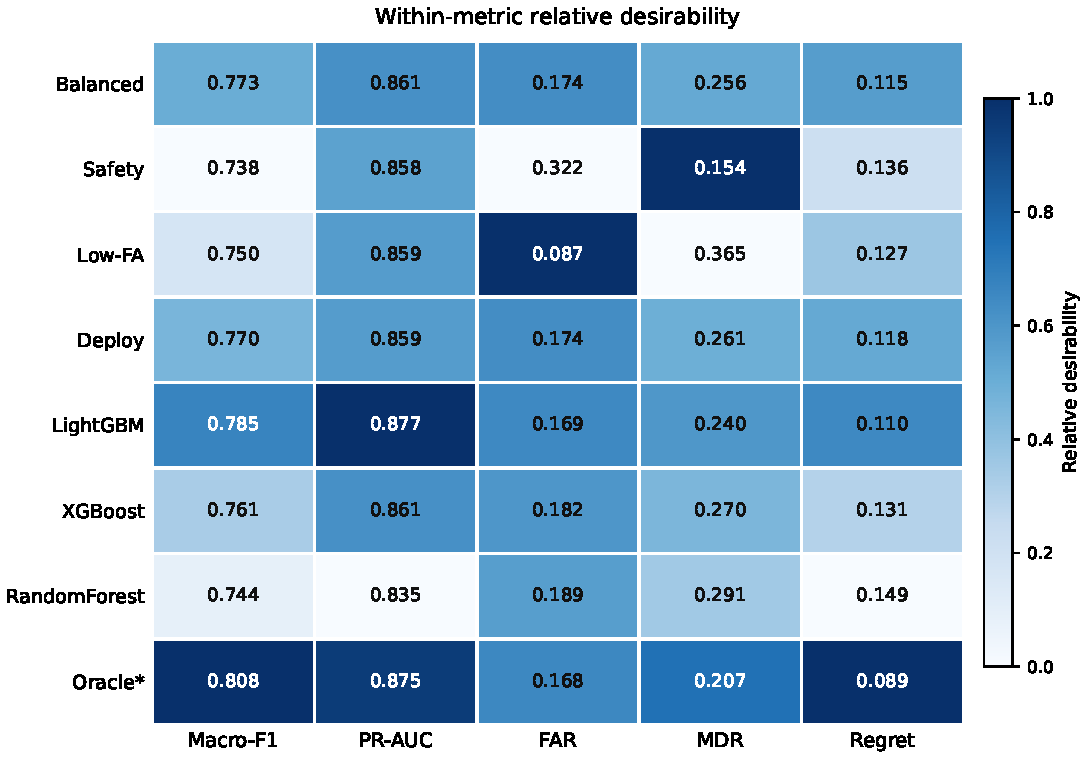
\includegraphics[width=0.98\linewidth]{figures/fig2_utility_heatmap_v20.pdf}
\caption{Core operating evidence for fixed and framework strategies. Colors encode within-column relative desirability and cell values show the reported metric values. For FAR, MDR and regret, lower values are mapped to higher relative desirability; for macro-F1 and PR-AUC, higher values are mapped to higher relative desirability. Color intensity should not be compared across metrics as an absolute value; it only indicates within-metric desirability. Oracle* denotes the non-deployable Oracle-Best-Test-Utility reference.}
\label{fig:engineering-utility}
\end{figure}


\subsection{FAR/MDR operating constraints}



A FAR violation is counted when FAR exceeds $\alpha=0.40$. An MDR violation is counted when MDR exceeds $\beta=0.35$. A joint FAR/MDR violation is counted when either condition is violated, i.e., $\mathrm{FAR}>\alpha$ or $\mathrm{MDR}>\beta$. These thresholds are not universal safety limits; they are benchmark-level tolerances selected before test evaluation to compare operating-constraint violations across scenarios. A sensitivity check over $\alpha\in\{0.20,0.30,0.40\}$ and $\beta\in\{0.20,0.30,0.35\}$ is computed from the existing scenario-level FAR/MDR rows without rerunning any model. Across this tolerance grid, Fixed-\allowbreak LightGBM retained the lowest or near-lowest joint-violation behavior among balanced defaults, while Framework-\allowbreak Safety and Framework-\allowbreak Low-\allowbreak False-\allowbreak Alarm consistently shifted violations toward FAR and MDR, respectively. At the benchmark tolerance $\alpha=0.40$, $\beta=0.35$, joint violation rates were 0.232 for Fixed-\allowbreak LightGBM, 0.270 for Framework-\allowbreak Deployment, 0.290 for Framework-\allowbreak Balanced, 0.450 for Framework-\allowbreak Low-\allowbreak False-\allowbreak Alarm and 0.480 for Framework-\allowbreak Safety. Test data are not used to tune model thresholds.

For RQ2, FAR/MDR analysis shows why a single accuracy-oriented winner is insufficient. Framework-\allowbreak Safety produced lower mean MDR (0.154) but increased mean FAR (0.322). Its safety utility was significantly higher than Fixed-\allowbreak LightGBM. This strategy is appropriate when missed detections are more costly than false alarms, but it requires an alarm workflow that can tolerate more warnings.



Framework-\allowbreak Low-\allowbreak False-\allowbreak Alarm showed the opposite tradeoff. It reduced mean FAR to 0.087 but increased mean MDR to 0.365. Its low-false-alarm utility was significantly higher than Fixed-\allowbreak LightGBM. Fixed-\allowbreak LightGBM nevertheless had a strong joint FAR/MDR violation rate (0.232) and remains an attractive default when a simple balanced operating point is needed.

These results make the operating-point dependency explicit. In a human-supervised monitoring station, a higher FAR may be acceptable if the aim is to avoid missed critical failures. In a highly automated production line, repeated false alarms may be more costly than delayed manual inspection, and a low-false-alarm strategy may be preferable. The same base model can therefore be appropriate under one threshold strategy and inappropriate under another.



\begin{table}[!htbp]
\centering
\scriptsize
\setlength{\tabcolsep}{2.4pt}
\renewcommand{\arraystretch}{1.05}
\caption{FAR/MDR constraint violation rates. Lower violation rates are better; safety and low-false-alarm strategies intentionally trade one error type against the other.}
\label{tab:far-mdr-constraints}
\begin{tabularx}{\linewidth}{@{}>{\RaggedRight\arraybackslash}X*{5}{>{\centering\arraybackslash}p{0.095\linewidth}}@{}}
\toprule
Strategy & FAR viol. & MDR viol. & Joint viol. & FAR & MDR \\
\midrule
Framework-Balanced & 0.080 & 0.230 & 0.290 & 0.174 & 0.256 \\
Framework-Safety & 0.370 & 0.110 & 0.480 & 0.322 & 0.154 \\
Framework-Low-False-Alarm & 0.030 & 0.420 & 0.450 & 0.087 & 0.365 \\
Framework-Deployment & 0.070 & 0.220 & 0.270 & 0.174 & 0.261 \\
Fixed-LightGBM & 0.053 & 0.179 & 0.232 & 0.169 & 0.240 \\
Fixed-XGBoost & 0.074 & 0.179 & 0.242 & 0.182 & 0.270 \\
Fixed-RandomForest & 0.095 & 0.242 & 0.337 & 0.189 & 0.291 \\
\bottomrule
\end{tabularx}
\end{table}


\begin{figure}[!htbp]
\centering
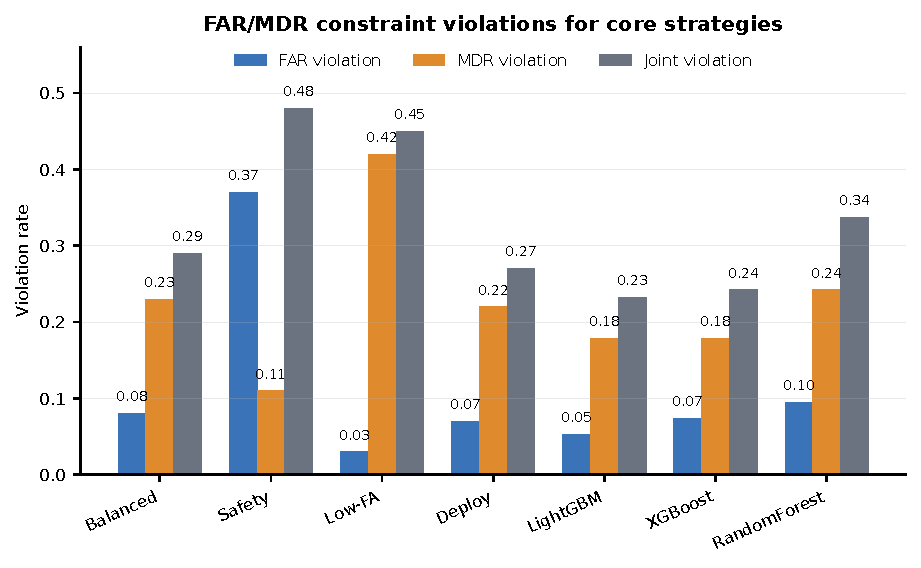
\includegraphics[width=0.98\linewidth]{figures/fig3_far_mdr_core_v19.pdf}
\caption{FAR/MDR constraint violation under the core strategy set used in the main comparison. Balanced, Safety, Low-FA and Deploy denote Framework-Balanced, Framework-Safety, Framework-Low-False-Alarm and Framework-Deployment, respectively. Lower values indicate fewer violations, but safety-oriented and low-false-alarm strategies encode different tradeoffs.}
\label{fig:far-mdr-violation}
\end{figure}




\subsection{Label-budget sensitivity}



For RQ3, label-budget sensitivity remains a limitation. The normal-only setting has no anomaly validation labels, so it cannot use validation macro-F1 to tune thresholds. It relies on normal-score quantiles or unsupervised calibration rules, while the 5\%, 20\% and full settings can use labeled validation subsets for utility-based threshold selection. For Framework-\allowbreak Balanced, the full-validation setting reached macro-F1 0.888, while the 20\% labeled, 5\% labeled and normal-only settings reached 0.715, 0.639 and 0.558, respectively. These results indicate that full validation labels remain valuable and that normal-only or very low-label settings are still difficult.



The label-budget criterion did not pass in the framework validation gate. Framework-Label-Budget selected the same model-threshold pairs as Framework-Balanced in the displayed label-budget scenarios, so Table~\ref{tab:label-budget-core} merges those rows. The results therefore do not support label-budget superiority or label-budget advantage. Label-budget analysis is presented as an engineering diagnostic that identifies when supervised tree baselines and validation thresholds remain necessary.

\begin{table}[!htbp]
\centering
\scriptsize
\setlength{\tabcolsep}{2.6pt}
\renewcommand{\arraystretch}{1.05}
\caption{Core label-budget sensitivity results. Normal-only calibration has no anomaly validation labels and therefore cannot use validation macro-F1 threshold tuning. Framework-Label-Budget selected the same model-threshold pairs as Framework-Balanced in these label-budget scenarios, so the rows are merged to avoid implying independent results.}
\label{tab:label-budget-core}
\begin{tabularx}{\linewidth}{@{}>{\RaggedRight\arraybackslash}p{0.33\linewidth}>{\RaggedRight\arraybackslash}p{0.13\linewidth}*{4}{>{\centering\arraybackslash}p{0.09\linewidth}}@{}}
\toprule
Strategy & Label budget & Macro-F1 & PR-AUC & FAR & MDR \\
\midrule
Fixed-LightGBM & 5pct & 0.632 & 0.701 & 0.255 & 0.464 \\
Fixed-LightGBM & 20pct & 0.720 & 0.828 & 0.236 & 0.322 \\
Fixed-LightGBM & full & 0.887 & 0.955 & 0.115 & 0.111 \\
Framework-Balanced / Label-Budget & normal\_\allowbreak{}only & 0.558 & 0.574 & 0.439 & 0.438 \\
Framework-Balanced / Label-Budget & 5pct & 0.639 & 0.712 & 0.197 & 0.503 \\
Framework-Balanced / Label-Budget & 20pct & 0.715 & 0.829 & 0.199 & 0.363 \\
Framework-Balanced / Label-Budget & full & 0.888 & 0.954 & 0.115 & 0.109 \\
\bottomrule
\end{tabularx}
\end{table}


The tabulated values show a monotonic gain from normal-only to full validation for Framework-\allowbreak Balanced/Label-\allowbreak Budget, reinforcing the value of labeled calibration data.

This negative result is practically important. It indicates that the evaluated candidate pool still benefits from labeled validation data for threshold calibration. The framework can organize the label-budget comparison, but it does not make normal-only calibration equivalent to supervised validation or convert limited-label calibration into a proven label-budget advantage. For engineering deployment, this suggests that collecting a small but representative validation set remains valuable.




\subsection{Robustness and domain shift}



Robustness and domain-shift analysis shows that the framework can be useful under stress protocols, but the evidence is bounded. Framework-\allowbreak Balanced achieved macro-F1 0.839 and robust utility 0.518 on robustness protocols. In domain-shift protocols, its macro-F1 was 0.615. Fixed-\allowbreak LightGBM remained strong, with macro-F1 0.834 under robustness protocols and 0.631 under domain-shift protocols.



\begin{table}[!htbp]
\centering
\scriptsize
\setlength{\tabcolsep}{2.4pt}
\renewcommand{\arraystretch}{1.05}
\caption{Core robustness and domain-shift results. Robustness and domain shift are reported separately because the framework audits domain-shift risk rather than solving it.}
\label{tab:robustness-domain-core}
\begin{tabularx}{\linewidth}{@{}>{\RaggedRight\arraybackslash}p{0.16\linewidth}>{\RaggedRight\arraybackslash}X*{5}{>{\centering\arraybackslash}p{0.075\linewidth}}@{}}
\toprule
Group & Strategy & Macro-F1 & PR-AUC & FAR & MDR & Utility \\
\midrule
robustness & Fixed-LightGBM & 0.834 & 0.916 & 0.171 & 0.160 & 0.503 \\
robustness & Framework-Balanced & 0.839 & 0.919 & 0.173 & 0.148 & 0.518 \\
robustness & Framework-Robust & 0.839 & 0.919 & 0.173 & 0.149 & 0.517 \\
domain shift & Fixed-LightGBM & 0.631 & 0.768 & 0.225 & 0.443 & -0.037 \\
domain shift & Framework-Balanced & 0.615 & 0.758 & 0.205 & 0.477 & -0.067 \\
domain shift & Framework-Robust & 0.615 & 0.758 & 0.205 & 0.477 & -0.067 \\
\bottomrule
\end{tabularx}
\end{table}


These results suggest that validation-selected strategies can help align model and threshold selection with missing-sensor or noisy conditions. They do not justify a broad robustness advantage claim over Fixed-\allowbreak LightGBM. Thus, the framework is more useful for selecting thresholds under local input corruption than for overcoming source-to-target domain shift. Domain-shift deployment should therefore prioritize local calibration and post-deployment monitoring rather than relying on the framework alone.

Domain shift and robustness are separated because they represent different risks. Missing sensors and noise stress test local corruption of the input stream. Source-to-target and leave-target-weight holdouts test whether the model and threshold remain useful when operating conditions change. The results show that both risks should be reported, because a model can be stable under missing channels but still lose performance under target-condition shifts.




\subsection{Prepared-input prediction latency and deployment-screening evidence}



The latency analysis reports prepared-input prediction latency on prepared features or prepared windows. It is not end-to-end robot-cell latency: sensor I/O, robot middleware, feature extraction for tree models, alarm handling and operator response are outside the measured path in the available artifacts. The values are reported per window, and prepared-input low-latency candidates must still be validated with end-to-end timing in the target robot cell.

Latency and model size affect deployability. Fixed-\allowbreak LightGBM and Fixed-\allowbreak XGBoost had low mean latencies (0.0064 ms and 0.0059 ms, respectively), while Fixed-\allowbreak RandomForest was slower (0.1970 ms). Framework-\allowbreak Deployment had mean latency 0.0504 ms and included latency and model-size penalties in its validation utility. Framework-\allowbreak Deployment was significantly higher than Fixed-\allowbreak XGBoost on prepared-input deployment-screening utility (mean difference 0.0603, Wilcoxon p=2.14e-10) and higher than Fixed-\allowbreak RandomForest (mean difference 0.1175, Wilcoxon p=5.88e-11), but it was not significantly higher than Fixed-\allowbreak LightGBM.



Deep reconstruction baselines had low measured latency in this benchmark, for example AutoEncoder latency 0.0024 ms, but their detection metrics were less stable under FAR/MDR constraints. Deployment decisions should therefore consider latency, model size, FAR and MDR jointly.

Latency alone is not a sufficient screening criterion. A fast model that produces unstable thresholds or a high missed-detection burden is not automatically preferable. Conversely, a slower model can still be acceptable if it runs within the cycle time of the monitoring system and reduces the operational cost. The prepared-input deployment-screening utility is therefore treated as a screening score over prepared inputs rather than as real deployment validation.



\begin{table}[!htbp]
\centering
\scriptsize
\setlength{\tabcolsep}{2.4pt}
\renewcommand{\arraystretch}{1.05}
\caption{Prepared-input prediction latency and deployment-screening summary. The prepared-input deployment-screening utility combines detection metrics with explicit latency and size penalties; it is not a field-deployment validation metric.}
\label{tab:latency-deployment}
\begin{tabularx}{\linewidth}{@{}>{\RaggedRight\arraybackslash}X*{5}{>{\centering\arraybackslash}p{0.092\linewidth}}@{}}
\toprule
Strategy & Latency ms & Size MB & Train s & Screen util. & Macro-F1 \\
\midrule
Framework-Deployment & 0.050 & 0.972 & 0.158 & 0.284 & 0.770 \\
Fixed-LightGBM & 0.006 & 1.000 & 0.153 & 0.326 & 0.785 \\
Fixed-XGBoost & 0.006 & 1.000 & 0.123 & 0.259 & 0.761 \\
Fixed-RandomForest & 0.197 & 1.000 & 0.228 & 0.202 & 0.744 \\
Fixed-AutoEncoder & 0.002 & 0.453 & 0.112 & -0.368 & 0.548 \\
Fixed-LSTM-AE & 0.004 & 0.046 & 0.195 & -0.463 & 0.485 \\
Fixed-USAD & 0.004 & 0.850 & 0.156 & -0.387 & 0.548 \\
\bottomrule
\end{tabularx}
\end{table}


\begin{figure}[!htbp]
\centering
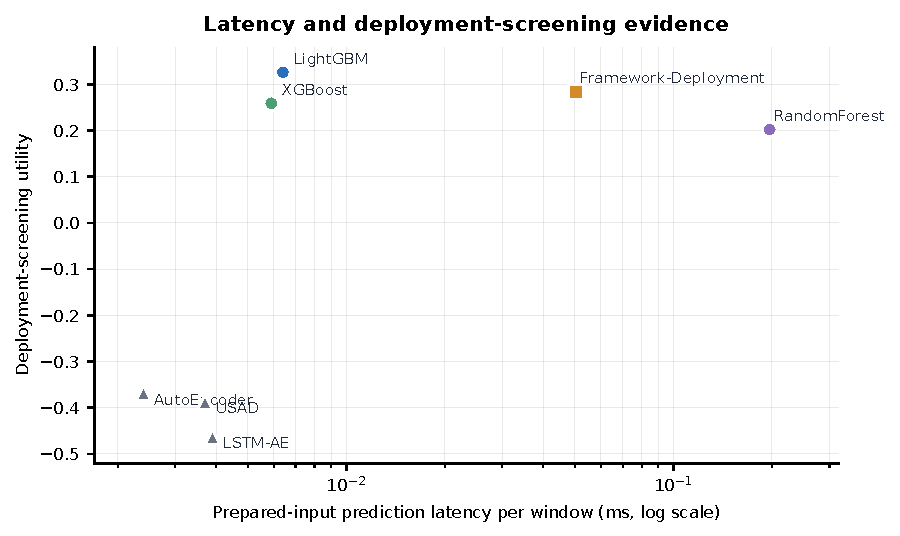
\includegraphics[width=0.98\linewidth]{figures/fig6_latency_scatter_v19.pdf}
\caption{Prepared-input prediction latency and deployment-screening utility for core strategies. The scatter plot avoids a dual-axis display; latency values are not end-to-end robot-cell latency and do not include sensor I/O, robot middleware, tree-model feature extraction, alarm handling or operator response.}
\label{fig:latency-deployment}
\end{figure}




\subsection{Model selection guidelines}



The framework often selected LightGBM or other strong tree baselines across engineering scenarios. This is an important result, not a weakness to hide. It indicates that the framework is a validation and calibration layer around a candidate pool, not a model that replaces strong baselines.



For label-rich settings, Framework-\allowbreak Balanced or Fixed-\allowbreak LightGBM is recommended. For label-scarce settings, Fixed-\allowbreak LightGBM with validation-only thresholding remains the safer default because label-budget superiority was not established. For safety-critical settings, Framework-\allowbreak Safety is preferred when a higher FAR can be tolerated. For low-false-alarm settings, Framework-\allowbreak Low-\allowbreak False-\allowbreak Alarm is preferred when missed detections are less costly. For low-latency candidate selection, Fixed-\allowbreak LightGBM or Fixed-\allowbreak XGBoost remains attractive.

The model-selection map should therefore be read as a decision audit rather than as evidence that the framework always chooses diverse models. In many scenarios, choosing LightGBM is the correct validation-supported decision. The framework adds value by documenting that choice and by identifying the conditions under which a safety, low-false-alarm or prepared-input deployment-screening utility changes the recommendation.





\begin{table}[!htbp]
\centering
\footnotesize
\setlength{\tabcolsep}{4pt}
\renewcommand{\arraystretch}{1.10}
\caption{Compressed application scenario mapping for operating-objective-specific strategy selection.}
\label{tab:application-scenario}
\begin{tabularx}{\linewidth}{@{}>{\RaggedRight\arraybackslash}p{0.25\linewidth}>{\RaggedRight\arraybackslash}p{0.30\linewidth}>{\RaggedRight\arraybackslash}X@{}}
\toprule
Scenario & Recommended strategy & Main caveat \\
\midrule
Safety-critical & Framework-Safety & FAR increases and alarm handling must be feasible. \\
Low false alarm & Framework-Low-False-Alarm & MDR increases and residual risk must be accepted. \\
Label-rich & Fixed-LightGBM / Framework-Balanced & No dominance over the strongest fixed baseline is claimed. \\
Label-scarce & Fixed-LightGBM & Low-label calibration remains weak. \\
Domain shift & Fixed-LightGBM / local calibration & The framework audits risk rather than solving shift. \\
Low-latency screening & LightGBM / XGBoost & End-to-end robot-cell timing validation is still required. \\
\bottomrule
\end{tabularx}
\end{table}






\section{Engineering Discussion}

The central engineering distinction is between benchmark ranking and deployment decision support. A benchmark can identify Fixed-\allowbreak LightGBM as a strong model, but it does not by itself specify the operating threshold when missed detections, nuisance alarms, calibration labels, robustness stress and CPU latency carry different costs. The framework turns the benchmark outputs into a pre-deployment audit: the operating objective is fixed before test evaluation, model-threshold selection is performed on validation data only and final test metrics document the consequences of that decision.

Frequent selection of LightGBM is therefore an engineering finding rather than a weakness. A reliable prepared-input low-latency candidate is valuable for subsequent robot-cell validation. The framework adds value by verifying that default under leakage-safe splits, calibrating its threshold and identifying when a cost-specific strategy changes the recommendation. The safety and low-false-alarm strategies illustrate this role: reducing MDR is useful for safety-critical inspection workflows but increases FAR, while reducing FAR is useful for production lines sensitive to nuisance stops but increases MDR.

Offline validation remains only a pre-deployment gate. It is closer to deployment than test-set threshold tuning, but it cannot guarantee behavior under new robot programs, sensor aging, maintenance changes or operator response loops. The framework is therefore best used before field deployment: engineers define an operating cost, run leakage-safe validation on representative calibration data, select the model-threshold pair for that cost and then review FAR, MDR, latency and robustness evidence before online testing.

This framing provides a reproducible engineering protocol, utility definitions, statistical evidence, scenario guidance and negative-result boundaries for deployment-oriented anomaly monitoring. It audits domain shift and robustness risks; it does not claim to solve them.


\subsection{Answers to the research questions}
RQ1 shows a bounded result: validation-only model-threshold selection improves operating utilities over weaker fixed baselines such as Fixed-\allowbreak XGBoost and Fixed-\allowbreak RandomForest in several objectives, but it does not reduce balanced regret relative to the strongest fixed baseline, Fixed-\allowbreak LightGBM. RQ2 shows that Framework-\allowbreak Safety and Framework-\allowbreak Low-\allowbreak False-\allowbreak Alarm improve their corresponding utilities over Fixed-\allowbreak LightGBM, whereas Fixed-\allowbreak LightGBM remains the preferred default for balanced and several deployment-oriented settings. RQ3 shows that label budget, missing sensors, domain shift and latency constraints materially change the deployment recommendation; label-budget superiority is not established, and domain shift remains an audited risk.


\section{Limitations and Threats to Validity}

This study is intentionally framed as an engineering evaluation and decision framework. It does not propose a new anomaly detection algorithm and does not show universal model dominance over Fixed-\allowbreak LightGBM. Fixed-\allowbreak LightGBM remains a strong default across several metrics and deployment scenarios, and that result is part of the evidence rather than an inconvenience. The framework should therefore be judged by whether it makes model-threshold choices auditable under stated constraints, not by whether it replaces the strongest baseline in every setting.

Label-budget superiority was not established. Normal-only and 5\% labeled validation settings remained difficult, and the results should not be interpreted as solving low-label anomaly detection. Domain shift also remains challenging: source-to-target and leave-target holdouts still reduced performance, and the framework should be treated as a way to audit this risk rather than eliminate it.

Dataset scope is another limitation. RoAD is used only as secondary stress evidence because previous protocol audits identified confounding and artifact risks. NIST UR and KUKA are not used as primary binary evidence in the main analysis because their labels, access pattern or task structure do not support the same robotic-arm binary protocols. The evidence therefore supports a bounded diagnostic framework, but further industrial datasets and online robot-cell deployment would be needed to assess generality in production.



The deep reconstruction baselines use compact fixed configurations and limited training epochs for reproducible benchmarking rather than architecture optimization. Stronger tuning may improve their standalone performance, but it would not change the framework's role as a validation-only model-threshold selection layer.

The framework is bounded by its candidate model pool. If every eligible model fails under a new operating condition, validation-based selection cannot recover performance. Utility weights also require engineering justification. The safety and low-false-alarm utilities used here encode plausible but simplified preferences; a plant may need different weights based on downtime cost, inspection labor, safety risk, spare-part availability and production schedule. Such weights should be fixed before test evaluation and documented in the deployment protocol.


\section{Conclusion}



This study evaluates a leakage-safe and calibration-aware engineering framework for robotic-arm multi-sensor anomaly diagnosis. The framework compares fixed models and validation-selected strategies under FAR/MDR, domain-shift, missing-sensor, label-budget and latency constraints.



Across the evaluated strategy-validation scenarios, Fixed-\allowbreak LightGBM remained the strongest balanced default with macro-F1 0.785 and PR-AUC 0.877. Framework-\allowbreak Safety reduced MDR to 0.154 at FAR 0.322, whereas Framework-\allowbreak Low-\allowbreak False-\allowbreak Alarm reduced FAR to 0.087 at MDR 0.365.

The main finding is not that a new detector outperforms all baselines. Strong tree baselines, especially Fixed-\allowbreak LightGBM, are often reliable. Scenario-specific strategies can nevertheless align model and threshold choice with operational cost. Safety and low-false-alarm strategies showed statistically supported utility improvements over Fixed-\allowbreak LightGBM for their respective objectives, whereas balanced, robust and prepared-input deployment-screening utilities did not establish universal model dominance over Fixed-\allowbreak LightGBM.



These results support a bounded and practical engineering contribution: a reproducible protocol and decision framework for deployment-oriented decisions in robotic anomaly monitoring. The claim is explicitly separated from algorithmic novelty or universal model-dominance claims.




\section*{Funding}
This work was supported by grants from FDCT-MOST (0018/2025/AMJ) and Macao Polytechnic University (RP/FCA-25/2025).

\section*{Declaration of competing interest}
The authors declare that they have no known competing financial interests or personal relationships that could have appeared to influence the work reported in this paper.

\section*{Data availability}
The public datasets used in this study are available from their original repositories, including IMAD-DS and RoAD, subject to their access and redistribution terms. Where redistribution is permitted, dataset copies or processed artifacts are included in the public reproducibility repository. Where redistribution is restricted or not verified, the repository provides official download instructions, expected file trees, checksums where available, preprocessing scripts and data-placement templates. Aggregated result tables, split summaries, FAR/MDR sensitivity outputs, statistical comparison tables, command manifests and figure/table source data are provided in the Supplementary Material and public reproducibility repository: [repository link to be added before submission].

\section*{Code availability}
The scripts used for benchmark aggregation, threshold analysis, statistical comparison, cluster-bootstrap analysis, FAR/MDR sensitivity analysis, table generation and figure generation are provided in the public reproducibility repository: [repository link to be added before submission]. Dataset-adapter scripts are included when they do not redistribute restricted dataset content; adapters requiring local dataset copies are documented with data-placement instructions.

\section*{CRediT authorship contribution statement}
Haochen Li: Conceptualization, Methodology, Software, Validation, Formal analysis, Data curation, Writing -- original draft, Visualization.
Junhao Wei: Conceptualization, Methodology, Software, Validation, Formal analysis, Data curation, Writing -- review \& editing, Visualization.
Dexing Yao: Methodology, Software, Validation, Formal analysis, Data curation, Writing -- review \& editing, Visualization.
Yifu Zhao: Methodology, Software, Validation, Investigation, Data curation, Writing -- review \& editing.
Yanxiao Li: Methodology, Validation, Investigation, Data curation, Writing -- review \& editing.
Zhaoyan Mai: Methodology, Validation, Investigation, Data curation, Visualization, Writing -- review \& editing.
Jiamu Yu: Software, Validation, Formal analysis, Data curation, Writing -- review \& editing.
Baili Lu: Validation, Formal analysis, Investigation, Visualization, Writing -- review \& editing.
Sio-Kei Im: Conceptualization, Methodology, Supervision, Resources, Writing -- review \& editing.
Xu Yang: Conceptualization, Methodology, Supervision, Resources, Project administration, Writing -- review \& editing.
Yapeng Wang: Conceptualization, Methodology, Supervision, Project administration, Funding acquisition, Resources, Writing -- review \& editing.

\section*{Acknowledgements}
The authors acknowledge Macao Polytechnic University for institutional support.

\section*{Declaration of generative AI and AI-assisted technologies in the writing process}
During the preparation of this work, the authors used AI-assisted tools for language polishing, editing support and manuscript-organization assistance. The authors reviewed and edited the content and take full responsibility for the content of the published article.

\bibliographystyle{elsarticle-num}
\bibliography{references_v20}

\end{document}
